\chapter{Results}
\label{results}

\section{Investment strategies}
\subsection{Default lifecyccles}
As was discussed in the previous chapter, our individual decides between investing in risky (stocks) or risk-free (bonds) assets. The default allocations for share of risky asset are given by:

\begin{itemize}
	\item $100-t$, for all $t$
	\item $\begin{cases} 100\%, & t<40\\(200-2.5t)\%, & t\in[40,57]\end{cases}$
	\item $63\%$, for all $t$
	\item $30\%$, for all $t$
\end{itemize}

where the latter two are Markowitz's solution and Anadolu Hayat's moderate investment option respectively. Since we are only interested in age span between 28 and 57, Figure 4.9 shows the risky asset share $\pi_t$ only for that interval. 

\begin{figure}[h]
	\centering
	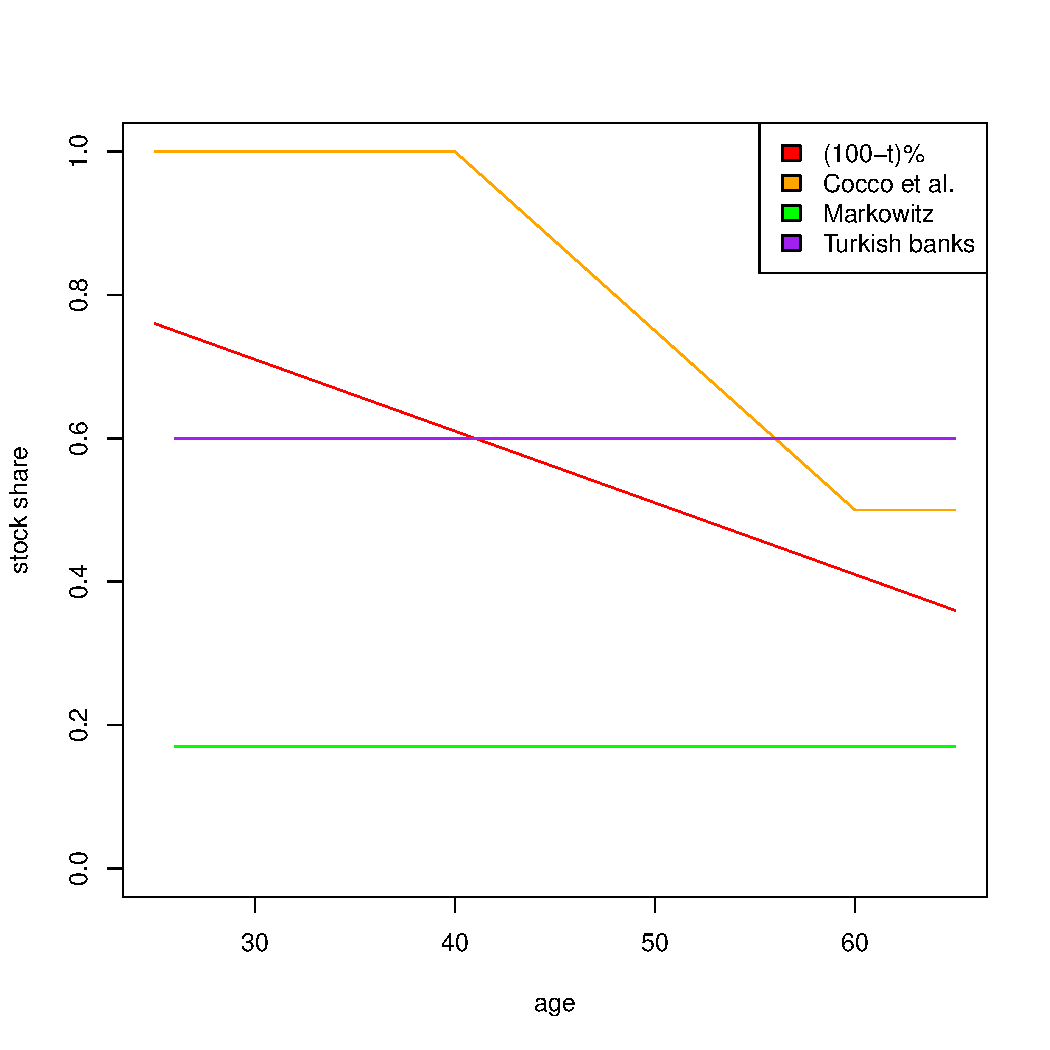
\includegraphics[scale=0.6]{figs/defaults.pdf}
	\caption{Default portfolio allocations of stock investments}
\end{figure}


\subsection{Individualized lifecycles}

To derive individualized lifecycle strategies, we used Merton's (1971) and Munk's (2016) optimal portfolio allocation formulas mentioned in chapters 2 and 3. Since these formulas depended on intratemporal amounts of capital, we have constructed three human capital series corresponding to flat, moderate and steep wage growth curves mentioned in the previous section. Figure 4.10 illustrates the risky asset shares given by Merton and Munk. 

\begin{figure}[h]
	\centering
	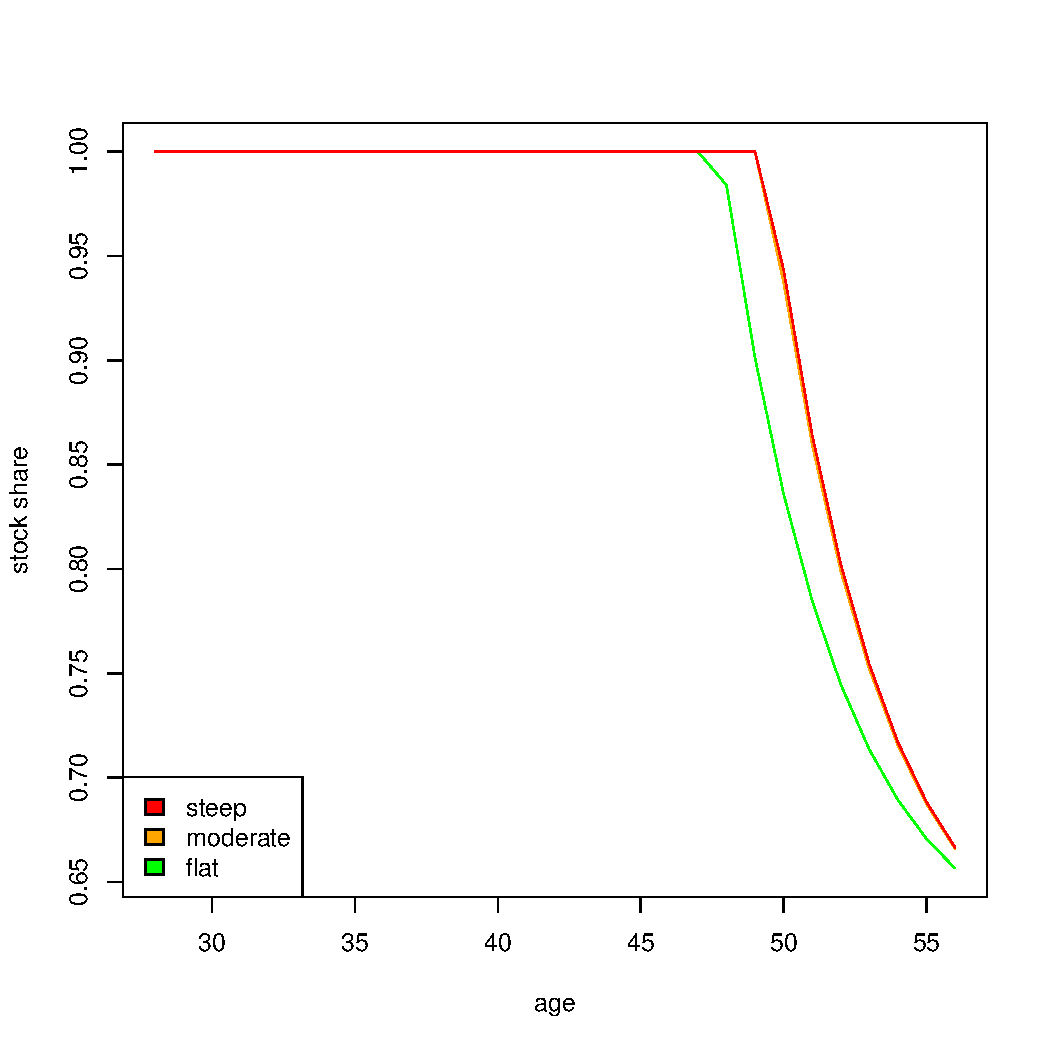
\includegraphics[scale=0.6]{figs/individuals.pdf}
	\caption{Individual portfolio allocations of stock investments}
\end{figure}

\section{Welfare comparison}


